\section*{c}

By using the rotation to imaginary time aka inverse temperature, it becomes possible to deal with the path integral (\ref{eq:1}) numerically. Suppose $\hbar=k_b=m=\omega=1$. Upon Wick rotation $\Delta t\rightarrow -ia,t\rightarrow-i\tau$, our path integral takes the form

\begin{equation}
    \langle x'=x_N,t'=t_N|x=x_0,t=t_0\rangle = \int_{x(\tau)=x}^{x(\tau')=x'}\mathcal{D}x\exp\left[-\sum_{i=1}^{N}a\left(\frac{(x_{i}-x_{i-1})^2}{2a^2}+\frac{x_i^2}{2}\right)\right]
\end{equation}

In order not to deal with the boundary conditions, we can trace over them, obtaining an analog of the partition function $Z$, which can then be used to calculate the expectation values of different operators. In particular, we will be interested in the energy of the ground state of the harmonic oscillator that, by a virial theorem, is simply given by the $\langle\hat{x}^2\rangle$. In terms of the path integral, we have

\begin{equation}
    \langle\hat{x}^2\rangle = \frac{(\Pi_{i=0}^{N-1}\int \mathrm{d}x_i)x_j^2\exp\left[-\sum_{i=1}^{N}a\left(\frac{(x_{i}-x_{i-1})^2}{2a^2}+\frac{x_i^2}{2}\right)\right]}{(\Pi_{i=0}^{N-1}\int \mathrm{d}x_i)\exp\left[-\sum_{i=1}^{N}a\left(\frac{(x_{i}-x_{i-1})^2}{2a^2}+\frac{x_i^2}{2}\right)\right]}
\end{equation}

We can simulate the $x_j$ by sampling from N-dimensional space, with Metropolis algorithm. 

\begin{figure}
    \centering
    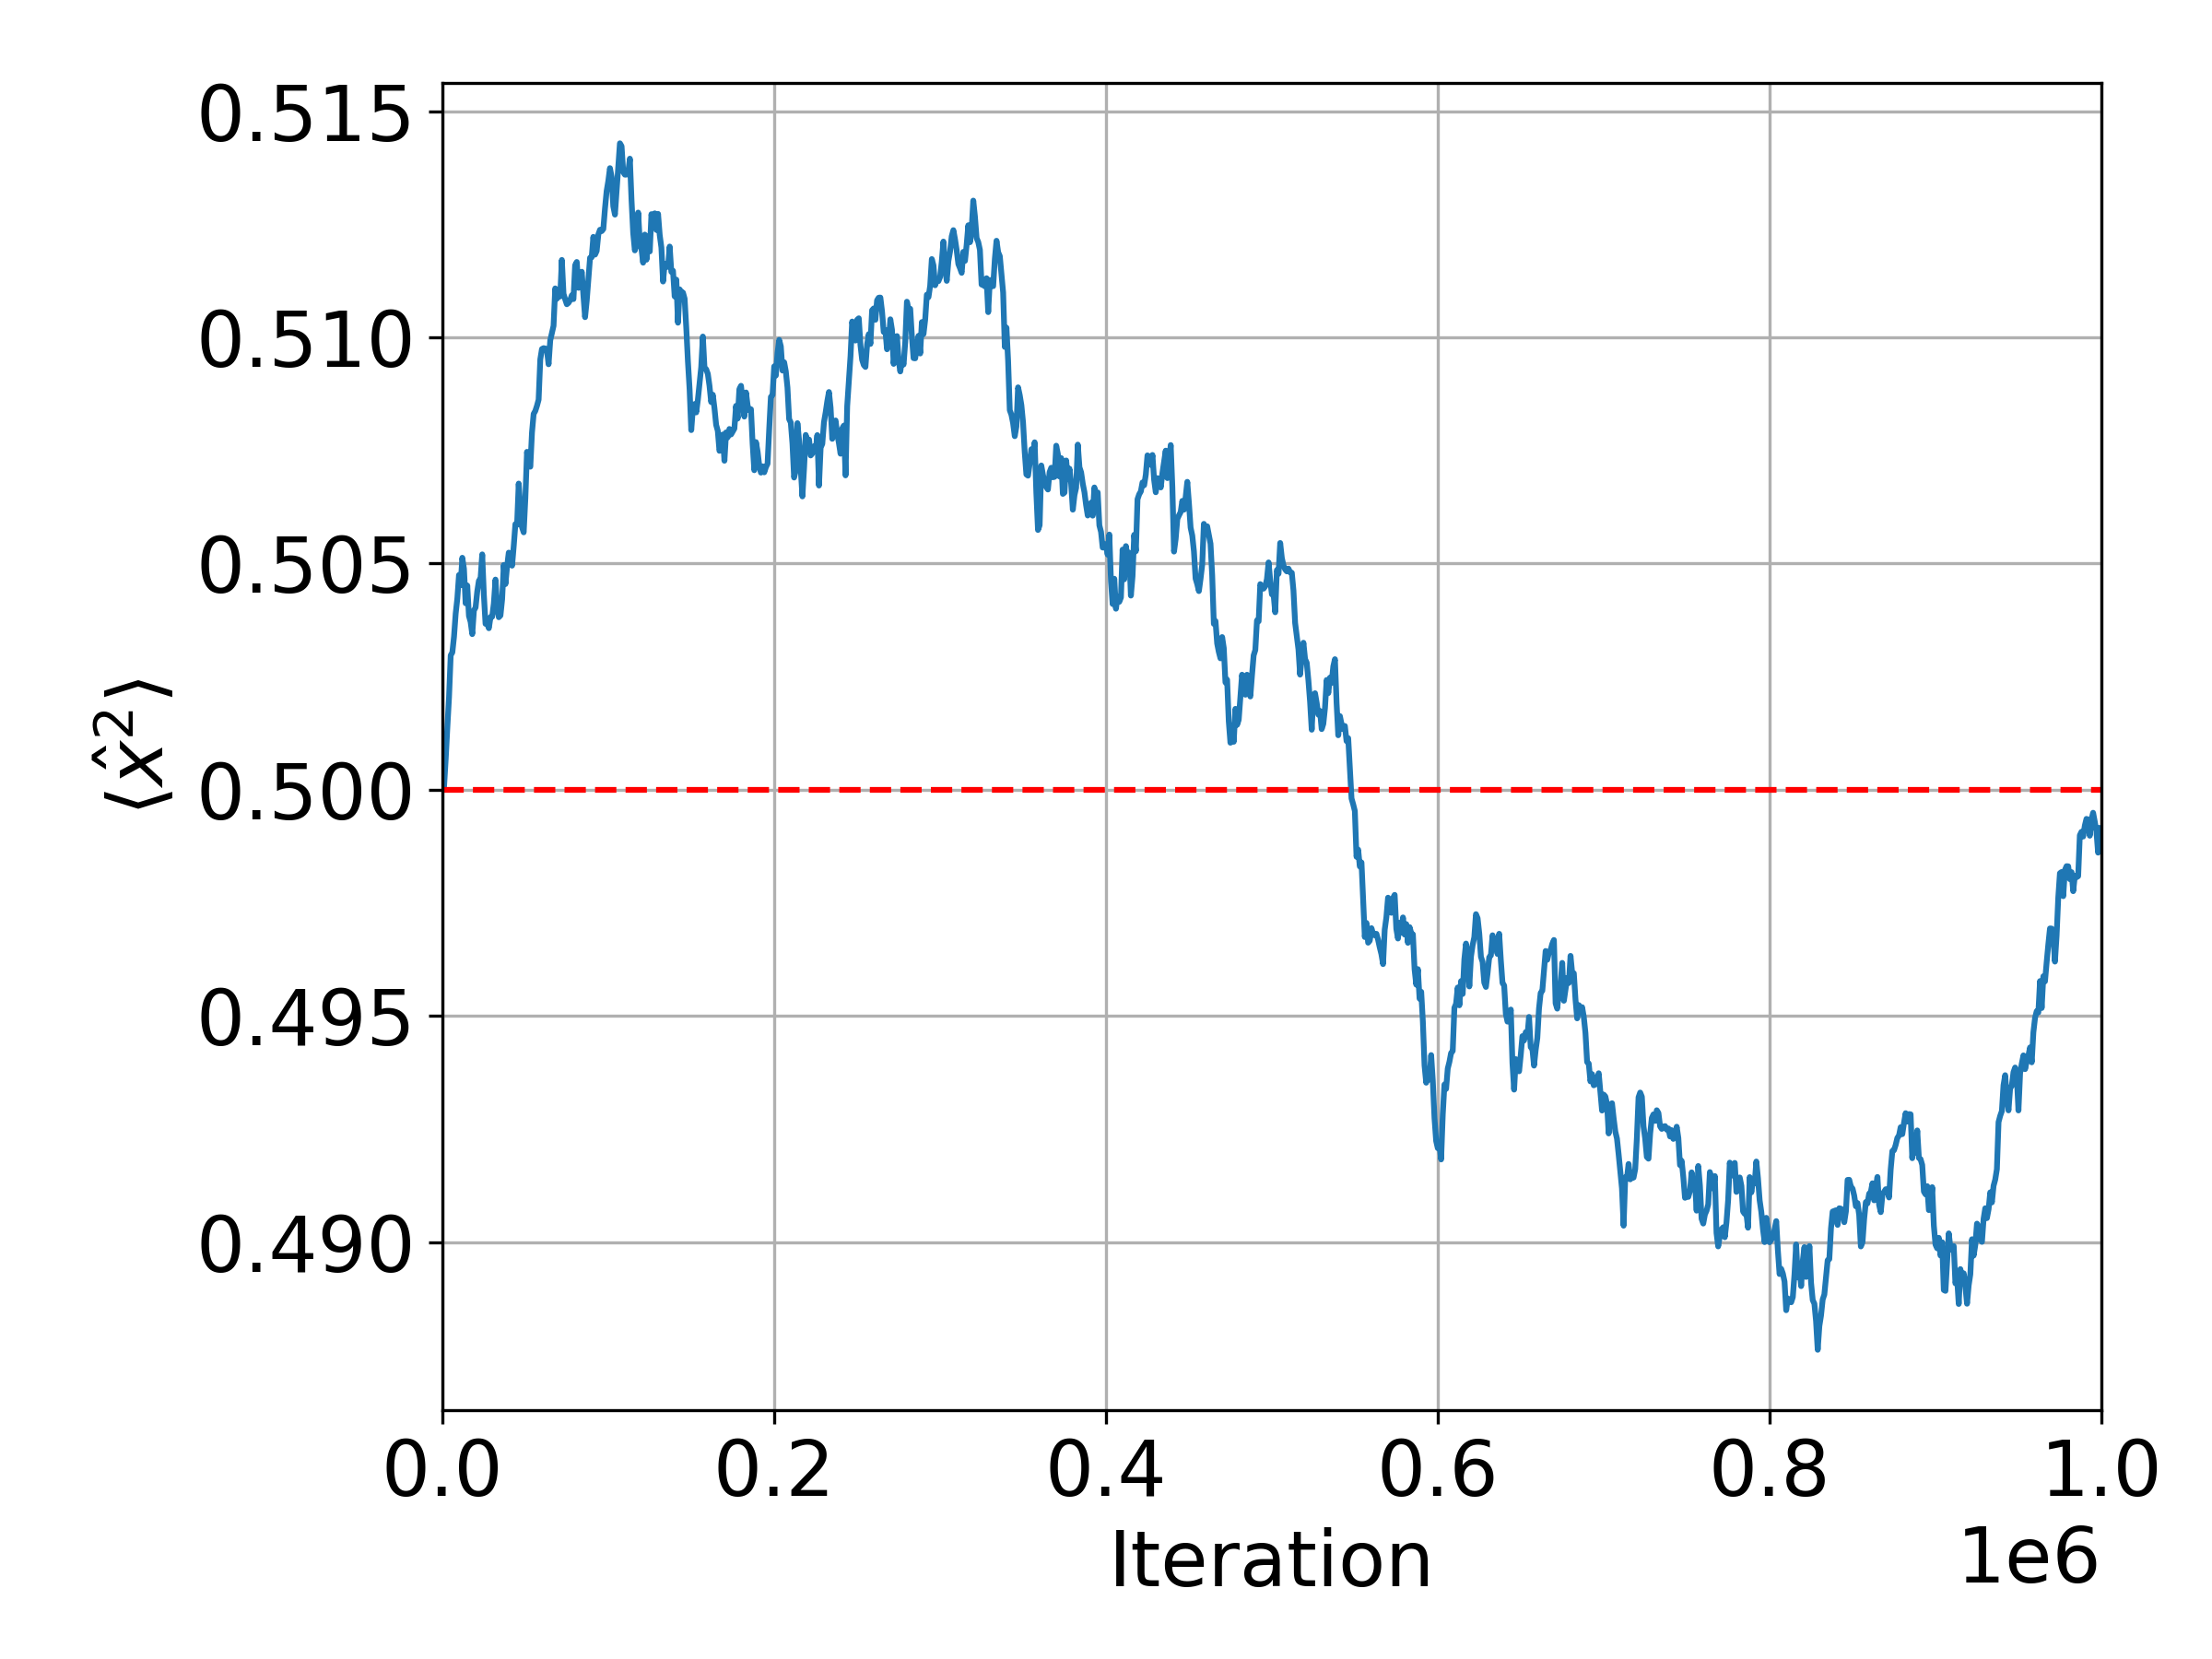
\includegraphics[width=0.6\linewidth]{figures/iterations.png}
    \caption{$\langle\hat{x}^2\rangle$ of N $x_j^2$ as function of iteration(the number of sweeps) through Metropolis algorithm\label{fig:1}}
\end{figure}

The predicted value of $\langle\hat{x}^2\rangle$ in low temperature limit from \ref{eq:3} is $0.5$, while the figure below shows the simulated $\langle\hat{x}^2\rangle$.

\begin{figure}
    \centering
    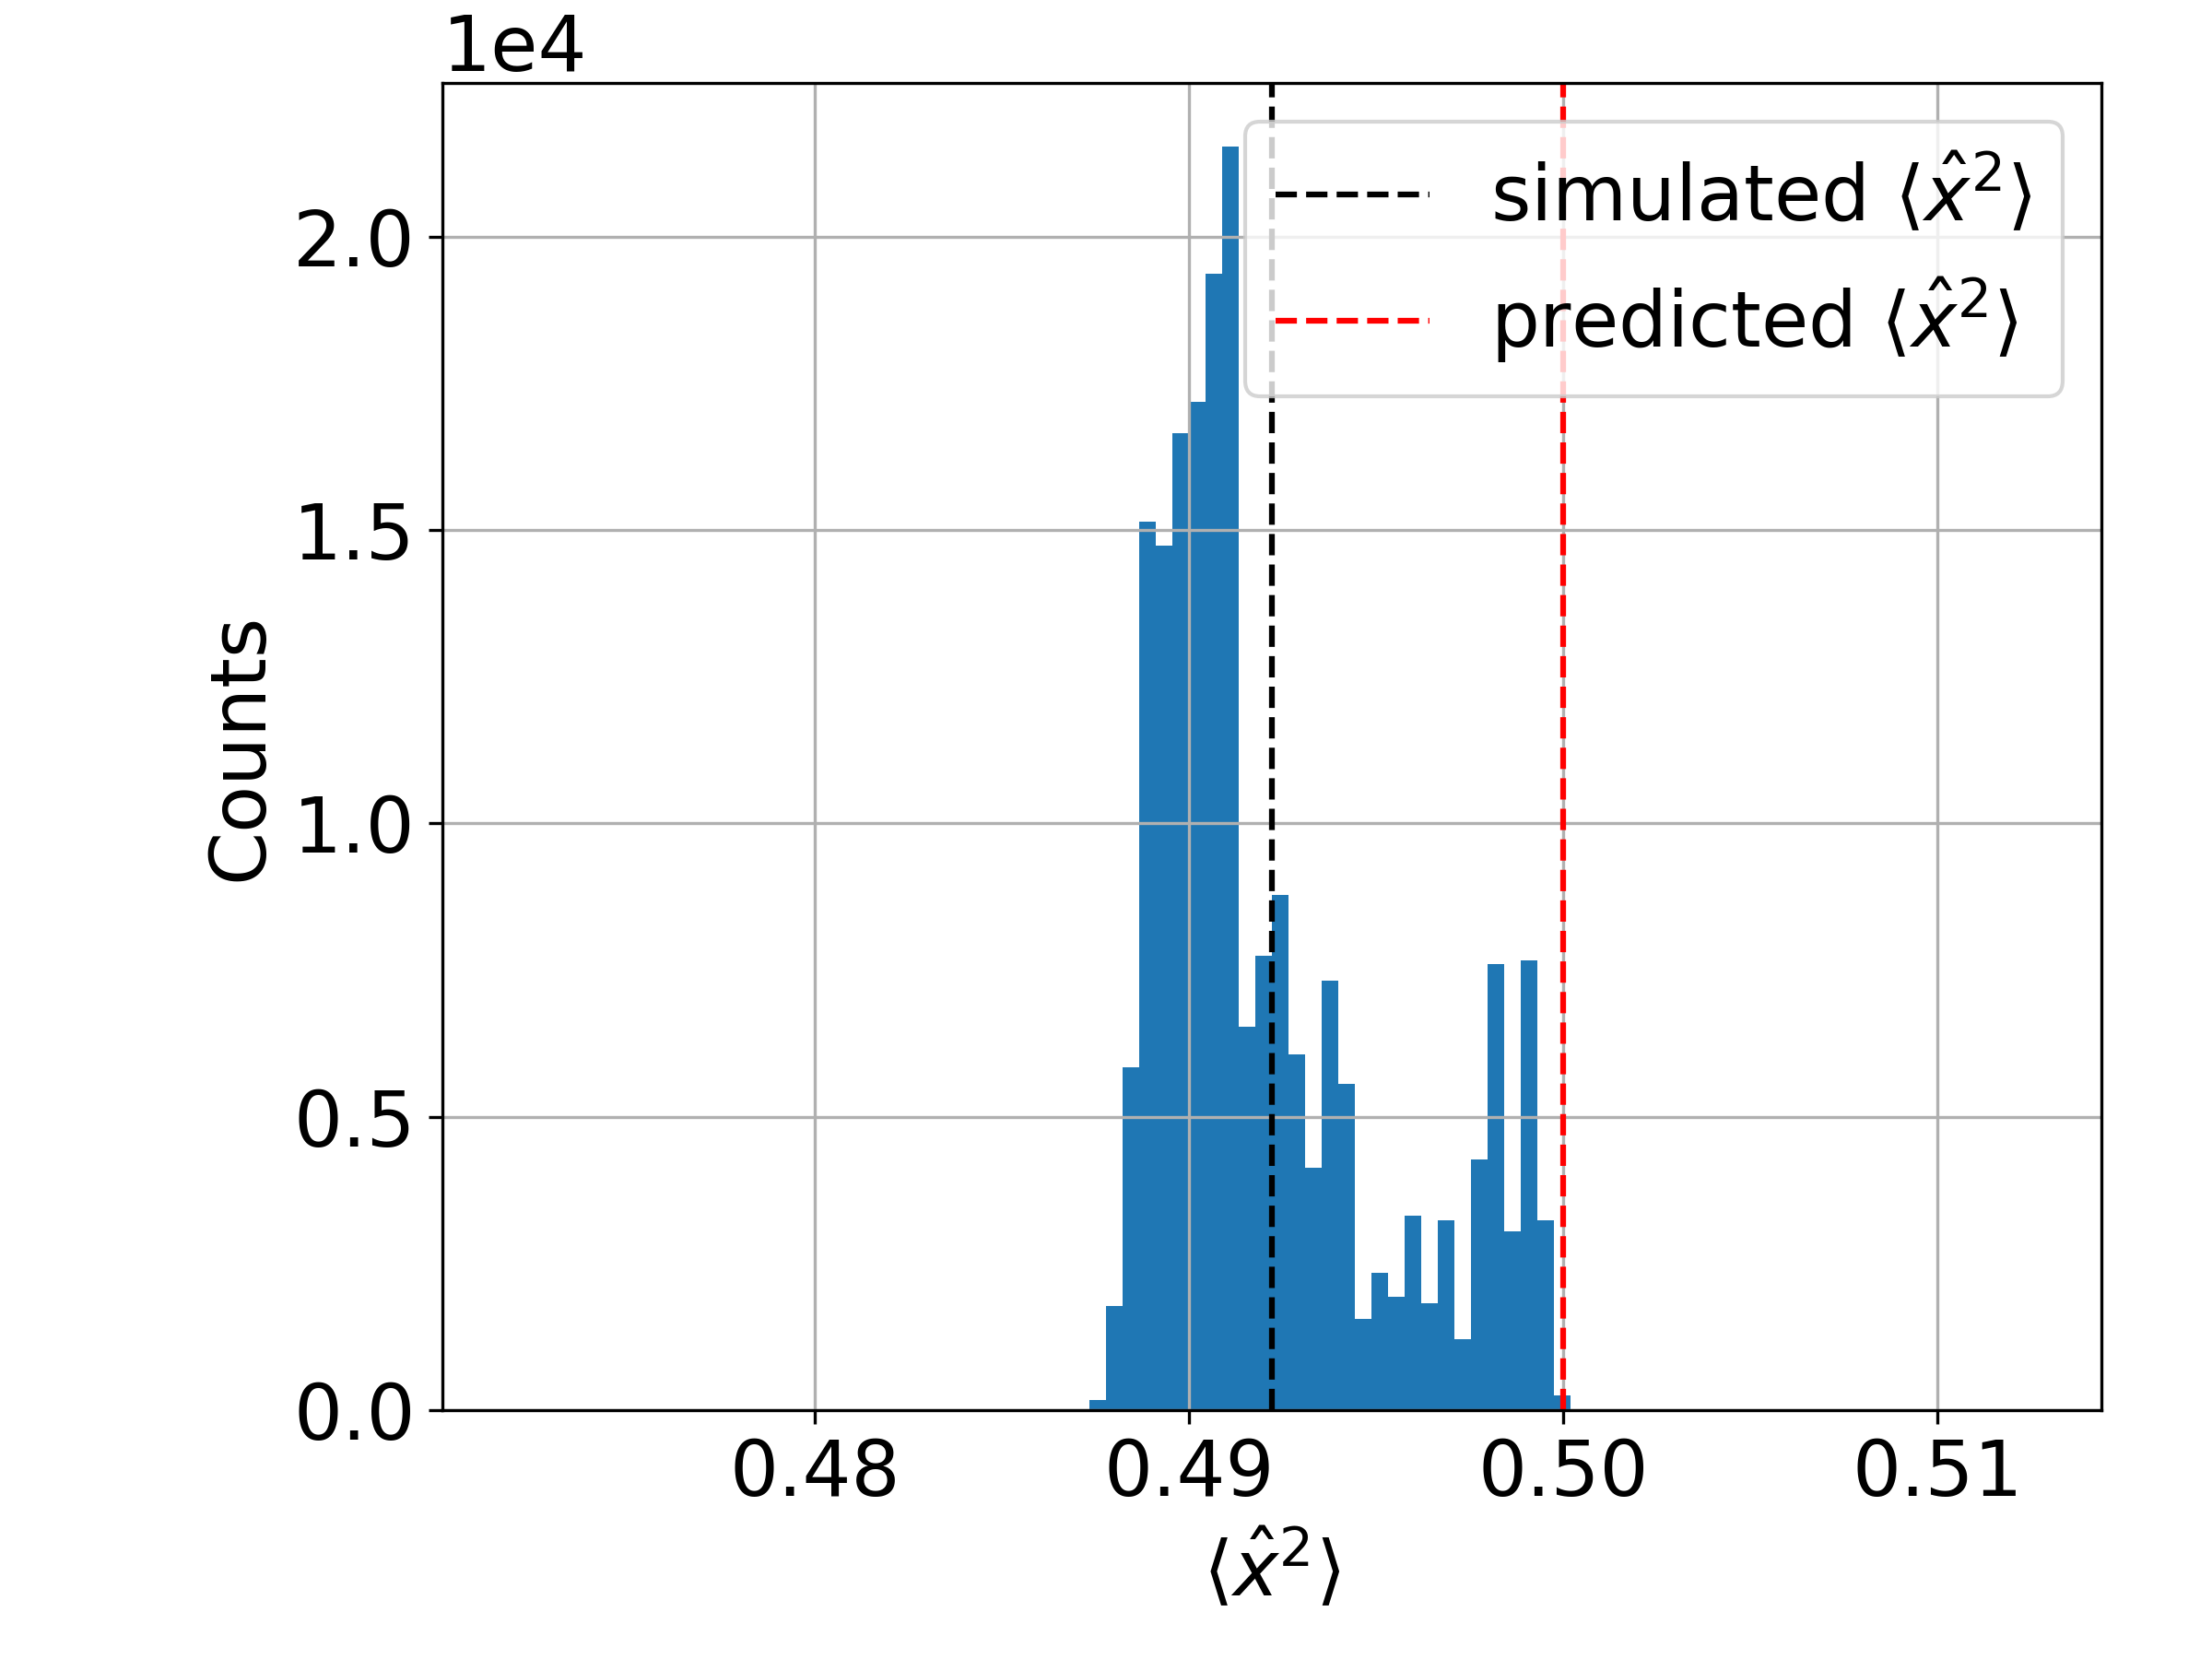
\includegraphics[width=0.6\linewidth]{figures/x2_hist.png}
    \caption{Comparison between simulated and predicted $\langle\hat{x}^2\rangle$}
\end{figure}

The difference between simulated and predicted $\langle\hat{x}^2\rangle$ is mainly due to statistical fluctuation and lack of number of sweeps. As we can see large fluctuation in Fig. \ref{fig:1}, more iteration is necessary. 

The code of these simulation is uploaded to a python notebook in GitHub\footnote{The source codes are available on GitHub \url{https://github.com/dachengx/QuantumHO/blob/main/simulation.ipynb}.}.
